\chapter{Описание моделей, отвечающих за генерацию поведения виртуального актора}


В данном разделе приводится теоретическое описание модели.

\section{Постановка задачи}
% тут описать то что обсуждали с А.В.
В рамках научно-исследовательской работы был расширен подход решения поставленной задачи задачи, который выражается в
использовании машинного обчучения. Данный подход используется в совокупности когнитивной архитектурой eBICA. 
eBICA – “emotional biologically inspired cognitive architecture” – “эмоциональная биологически вдохновленная когнитивная архитектура”. 

В этой архитектуре эмоциональные элементы добавлены практически ко всем процессам за счет модификации основных строительных блоков архитектуры. 
Ключевым моментом этой когнитивной архитектуры являются оценки, которые связаны со схемами и психическими состояниями как их атрибуты, 
моральные схемы, которые контролируют модели оценок и представляют социальные эмоции, а также семантические пространства, которые дают 
значения этих оценок.

Как видно из (Рис. \ref{pic:ris7}), архитектура представляет собой конгломерат компонентов: интерфейсный буфер, рабочая, процедурная, семантическая 
и эпизодическая системы памяти, система ценностей и система когнитивных карт \cite{Samsonovich01}. Три основных строительных блока для этих компонентов - это 
ментальные состояния, схемы и семантические карты. Семантическая память - это коллекция определений схем. Буфер интерфейса заполняется схемами.

\begin{figure}[h]
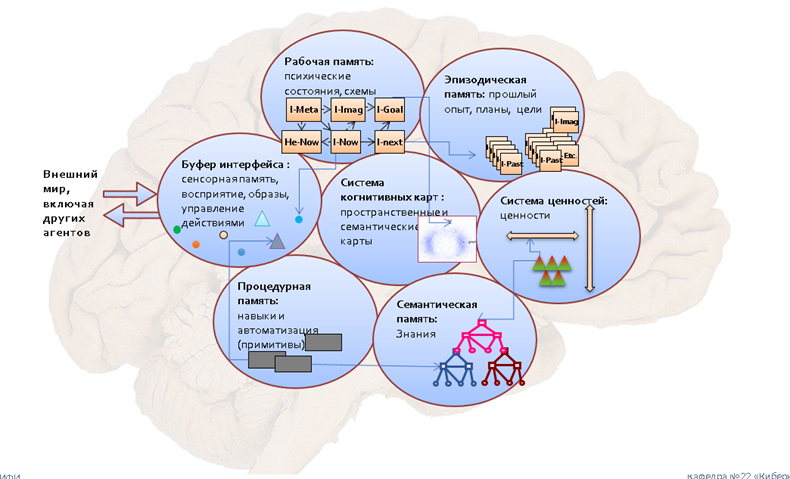
\includegraphics[width=0.75\columnwidth]{./img/ris7.png}
\centering  
\caption{Структура когнитивной архитектуры eBICA}
\label{pic:ris7}
\end{figure}

Рабочая память включает активные психические состояния. Эпизодическая память хранит неактивные психические состояния, сгруппированные 
в эпизоды - предыдущее содержимое рабочей памяти. Следовательно, эпизодическая память состоит из структур, аналогичных тем, которые 
обнаруживаются в рабочей памяти, но которые «заморожены» в долговременной памяти. Процедурная память включает в себя примитивы. Система 
ценностей включает в себя шкалы, представляющие основные значения. Система когнитивных карт включает, в частности, семантические карты 
эмоциональных ценностей. Семантическая карта использует абстрактное метрическое пространство (семантическое пространство) для представления 
семантических отношений между ментальными состояниями, схемами и их экземплярами, а также для присвоения значений их оценкам.


\section{Описание работы модели актора}

На момент начала выполнения работы уже была реализована система работы виртуальных агентов, и она состоит в том, что сперва 
считываются действия и объекты с заданными для них параметрами и значениями из Excel файла, а также инициализируются значения. 
Затем выбор действий происходит в следующем порядке: в радиусе вокруг оценок виртуального актора выбираются действия, которые 
попадают в этот радиус, а также проверяются различные условия, необходимые для выполнения действия. Если условия не выполняются, 
то действие не может быть выбрано. Затем, после того как в список добавлены все действия, которые могут быть выполнены, рассчитываются 
вероятности на основе оценок и рассчитанных констант. Также, если действие повторное, его вероятность несколько занижается. 
После расчета вероятностей выбирается действие, которое влияет на оценки виртуального актора. 

Помимо этого происходит замена состояний объектов и виртуальных акторов. После этого происходит перерасчет оценок Appraisals и Feelings \cite{Samsonovich01}.

Основная модель eBICA определяет поведение виртуального актора исходя из следующих факторов:

\begin{itemize}
  \item соматический;
  \item рациональный;
  \item когнитивный.
\end{itemize}

Нравственный фактор регулирует отношения первого актора со вторым на основе системы ценностей (представленной семантической картой) 
и моральных схем. Под когнитивным фактором понимается учет соображений нравственности, этики и морали, общей системы ценностей, 
понятий о добре и зле, о собственном достоинстве, эмпатии, соображений эстетики, стремлений к простоте и элегантности, и т.д. 
Учет этих соображений возможен на основе когнитивных оценок (appraisals) всех релевантных агентов, событий, их возможных действий 
и последствий этих действий, фактов, свойств, отношений, и т.д. Возможен вариант модели, в которой ответное действие может выбираться 
лишь из двух вариантов: положительная реакция на действие человека и отрицательная. Данная версия модели весьма неплохо работает даже 
с таким ограничением. Но невозможно придерживаться данной парадигмы при увеличении количества возможных вариантов для взаимодействия 
между акторами. В данной модели необходимо учесть пересчет оценок Appraisals и Feelings. Для пересчета оценок Appraisals используется 
следующая формула \ref{eq:appraisals01}:

\begin{equation}
  \begin{gathered}
    Appraisals=(1-r)*Appraisals+r*Action
    %P_{i+1j  } (R_{i+1j  } , {\varphi}_{i+1} , {\theta}_{j  }) \\
  \end{gathered}
  \label{eq:appraisals01}
\end{equation}

где Appraisals - оценка, 
r - эмпирически вычисленная константа экспоненциального затухания, 
Action - оценка совершаемого действия на семантической карте.

Одновременно с Appraisals пересчитываются так называемые “чувства” Feelings согласно режиму работы моральной схемы.
Аффективное пространство VAD – это трехмерное векторное пространство, точки которого соответствуют определенным эмоциональным 
состояниям, или аффектам, представленным триплетами значений (Valence, Arousal, Dominance). 
Существуют и сходные модели: PAD (Pleasure, Arousal, Dominance), EPA (Evaluation, Potency, Arousal) и другие. 
Здесь мы используем модель VAD. Соответственно, под «семантической картой» здесь часто понимается ее конкретная 
разновидность: аффективная карта (или когнитивная семантическая карта).

Шкалы имеют следующие значения:
\begin{itemize}
  \item dominance – варьируется при значении от 0 (покорность) до +1 (доминантность) и описывает соответствующие чувства; 
  \item valense – при значениях от -1 до 0 показывает уровень негатива или радости соответственно; 
  \item arousal – значения от -1 до 1 показывают уровень возбуждения (заинтересованности), к примеру, гнев по уровню возбуждения сильнее раздражительности, но слабее ярости. 
\end{itemize}

Оценки представлены в виде векторов на трехмерной семантической карте \cite{seman_karta}, \ref{pic:ris5}.
Моральная схема определяет общую установку на оценку поведения акторов, согласно их ролям и типу ситуации. 
Ее целью (как агента) является достижение и поддержание «нормального» положения дел, определенного набором Feelings. 
Вообще говоря, моральная схема состоит из двух частей: части, распознающей тип ситуации и осуществляющей привязку (binding),
и части, реализующей динамику схемы. В случае парадигмы актора можно считать, что моральная схема одна, уже привязана, и 
потому первая часть ее не актуальна.

Субъективные оценки (Feelings) генерируются по определенным правилам на основании истории объективных оценок и состояний системы. 
Грубо говоря, Feelings – это субъективное представление о том, каким оцениваемый актор является «на самом деле», и, следовательно, 
какого поведения от него нужно ожидать и на какое место его нужно ставить своим поведением. Следовательно, выбор поведения актора 
должен осуществляться так, чтобы приблизить Appraisals к Feelings. 

Значение Feelings определяет моральная схема, которая может работать в одном из трех режимов. 
Первый режим основывается на формуле \ref{eq:feelings01}:

\begin{equation}
  \begin{gathered}
    Feelings=beta*Appraisals
  \end{gathered}
  \label{eq:feelings01}
\end{equation}

где beta – эмпирически вычисленная константа. 

В данном режиме схема говорит, что если актор ведет себя хорошо, то к нему нужно относиться как к хорошему, и т.д. 

Цель данного процесса – распознать и классифицировать актора, выработать отношение к нему и приписать ему определенную роль во взаимоотношениях. 

В данном режиме моральная схема работает пока разница между квадратами норм Feeling и Appraisals не станет меньше некоторого значения.

Суть второго режима заключается в том, что значение Feeling фиксировано и экстремально по абсолютной величине, т.е. находится на сфере, 
ограничивающей семантическую карту (предположим, что есть такая сфера). Направленность вектора Feeling может быть либо произвольной, 
определенной предысторией, либо дискретной – вдоль одной из осей.

Третий режим состоит в том, что значения Feelings меняются \ref{eq:feelings02}, подстраиваясь под текущие значения Appraisals (здесь r1 может быть отличным от r): 

\begin{equation}
  \begin{gathered}
    Feelings=(1-r_1 )*Feelings+r_1*(Appraisal-Feelings)
  \end{gathered}
  \label{eq:feelings02}
\end{equation}

Соответственно значения Appraisals и Feelings как говорится в работе \cite{Samsonovich05} пересчитываются после каждого действия первого актора, направленного на второго актора.
Также пересчет оценок происходит после определения и совершения одним из акторов ответного или самостоятельного действия. 
В данном контексте под термином “самостоятельное действие” имеется в виду действие, основанное лишь на текущем состоянии мира и 
значений векторов Appraisals и Feelings акторов, отобрежнные на (Рис. \ref{pic:ris8}). 


\begin{figure}[h]
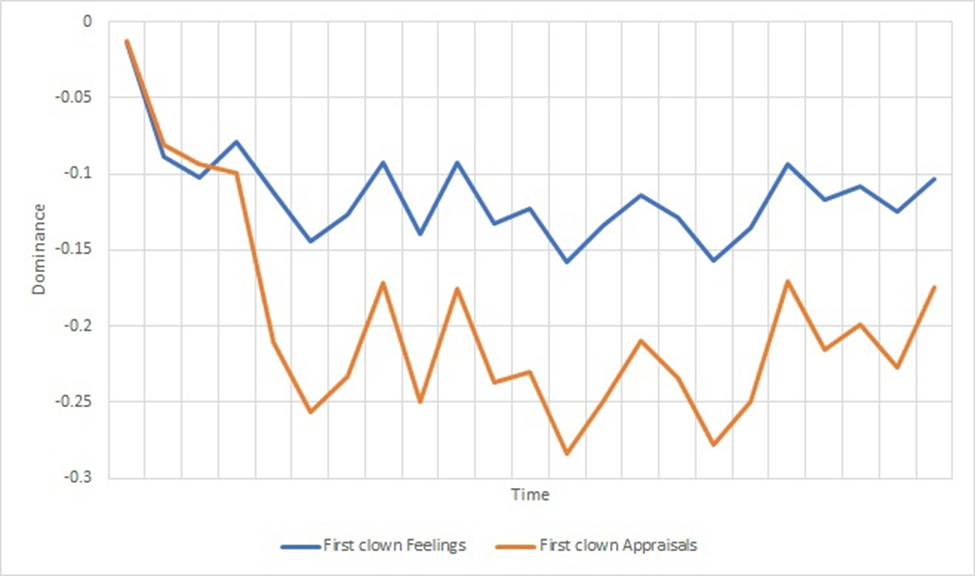
\includegraphics[width=0.75\columnwidth]{./img/ris8.png}
\centering
\caption{Корреляция значений Appraisals (оранжевая) и Feelings (синяя) для показателя доминантности на протяжении времени/действий с шагом в 5 секунд}
\label{pic:ris8}
\end{figure}

Согласно (Рис. \ref{pic:ris8}) мы видим, что работа модели сводится к выбору действия, 
которое будет максимально приближать Appraisals к Feelings и вектор соматического состояния к начальному положению.

\section{Способы распознавания речи}
Сейчас существует несколько методов решения задачи распознавания речи в аудиозаписи. Успешность и скорость их работы во многом зависит от дикции автора, качества записи аудиофайла, поданного на вход, фонового шума, а также от качества работы спроектированной системы распознавания, и, как следствие, от выбранного метода.

Разнообразие особенностей речи, а также реализуемых подходов к решению задачи распознавания ведут к многообразию существующих решений. Все они борются за лидерство по качеству работы, но все еще имеют свои индивидуальные достоинства и недостатки.

Самыми популярными методами распозвавания речи являются: 
\begin{itemize}
  \item Скрытое Марковское моделирование (HMM)
  \item Использование N-грамм
  \item Подход искусственного интеллекта
  \item Рекуррентные сети
\end{itemize}

До сих пор наиболее успешный \cite{1_speach} и часто используемый метод для распознавания речи - это математическая модель, полученная на основе модели Маркова (Рис. \ref{pic:speach_1}).
Скрытая Марковская модель представляет собой статистическую модель, моделирующую процесс Маркова с неизвестными параметрами. Пусть имеет N состояний модели. 
Каждое из состояний имеет свою вероятность наступления. Обозначим вероятности перехода между состояний как матрицу A=\{aij\}, где aij – вероятность перехода из i-го в j-е9
состояние. В каждом из своих состояний система принимает одно из M значений какого-то своего параметра. 

Обозначим вероятность выпадения каждого из M значений параметра в каждом из N состояний системы через B=\{bj(k)\}, 
где bj(k) – вероятность выпадения k-го значения параметра в j-м состоянии. Также введем вектор вероятности наступления начального состояния через 
π=\{πi\}, где πi – вероятность того, что в начальный момент система окажется в i-м состоянии. На рисунке \ref{pic:speach_1} представлена схема строения скрытой Марковской модели. 
Состояния представлены в виде голубых кружков (N штук), значения скрытого параметра представлены с помощью желтых квадратов (M штук). 
Каждая стрелка символизирует возможный переход и имеет свой вес (значение вероятности). Таким образом, скрытой Марковской моделью называется тройка λ = \{A, B, π\} \cite{2_speach}.

\begin{figure}[h]
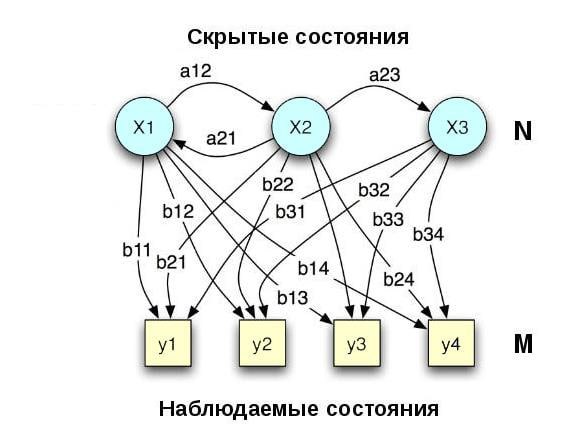
\includegraphics[width=0.75\columnwidth]{./img/speach_1.jpg}
\centering
\caption{Общая схема устройства скрытой Марковской модели. \cite{3_speach}}
\label{pic:speach_1}
\end{figure}

Использование скрытых Марковских моделей для распознавания речи основано на трех допущениях \cite{4_speach}:
\begin{enumerate}
  \item речь можно разбить на фрагменты (соответствующие состояниям в СММ) так, что внутри каждого фрагмента речевой сигнал можно рассматривать как стационарный. Параметры речи в его пределах постоянны;
  \item переход между состояниями осуществляется мгновенно;
  \item вероятность каждого фрагмента зависит только от текущего состояния модели и не зависит от предыдущих состояний.
\end{enumerate}

N-грамма – это модель представления данных, которая также может использоваться для распознавания речи \cite{5_speach}. 
N-граммная модель рассчитывает вероятность последнего элемента N-граммы при условии, что известны все предыдущие. 
В задаче распознавания речи элементами могут выступать фонемы, если задача решается на более низком уровне, или же целые слова. 

При использовании этого подхода предполагается, что появление каждого слова (фонемы) зависит только от предыдущих слов (фонем),
причем значение N указывает, от скольких предыдущих слов оно зависит. 


Вероятность фразы можно вычислить как произведение вероятностей каждого из слов этой фразы:

\begin{equation}
  \begin{gathered}
  P=P(\text{мой}) \times P(\text{дядя|мой}) \times P(\text{самых|мой дядя}) \times P(\text{честных|мой дядя самых}) \times P(\text{правил|мой дядя самых честных})
  \end{gathered}
  \label{eq:speach_formula_1}
\end{equation}

Здесь $P(\text{самых|мой дядя})$ обозначает условную вероятность возникновения «самых» при условии появления «мой дядя». Чтобы определить $P(\text{мой})$, нужно посчитать, сколько раз это слово встретилось в тексте, и поделить это значение на общее число слов. 
Рассчитать вероятность $P(\text{правил|мой дядя самых честных})$ уже сложнее. Чтобы упростить эту задачу, примем, что вероятность слова в тексте зависит только от предыдущего слова. Именно здесь проявляет себя выбранное значение N. 
Тогда формула для расчета фразы примет вид:

\begin{equation}
  \begin{gathered}
    P = P(\text{мой}) \times P(\text{дядя|мой}) \times P(\text{самых|дядя}) \times P(\text{честных|самых}) \times P(\text{правил|честных})
  \end{gathered}
  \label{eq:speach_formula_2}
\end{equation}

Рассчитать условную вероятность $P(\text{дядя|мой})$ несложно. Для этого считаем количество пар 'мой дядя', и делим на количество в тексте слова 'мой'. 
В результате, если мы посчитаем все пары слов в некотором тексте, мы сможем вычислить вероятность произвольной фразы. 
Этот набор рассчитанных вероятностей и будет биграммной моделью. Степень модели указывает на количество слов, учитываемых при расчете вероятностей. 
Рисунок \ref{pic:speach_2} показывает несколько N-грамм для небольших значений N. Униграмма имеет степень 1, биграмма – степень 2, триграмма – степень 3.

\begin{figure}[h]
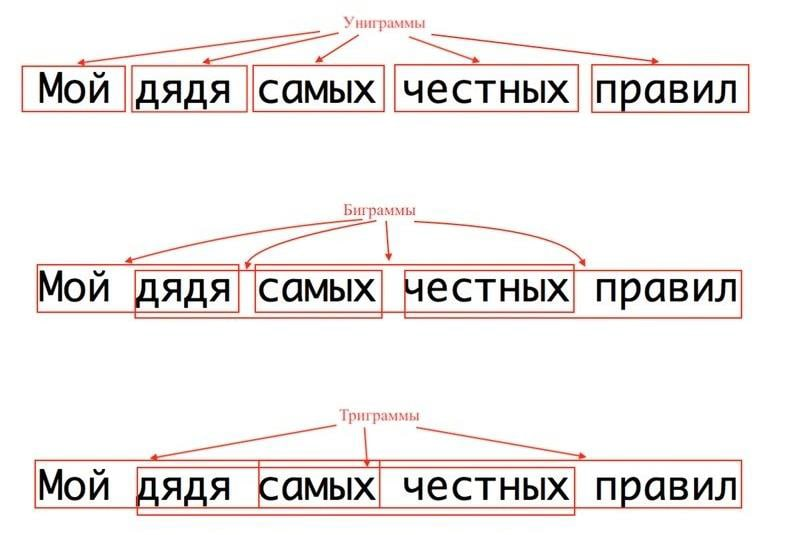
\includegraphics[width=0.75\columnwidth]{./img/speach_2.jpg}
\centering
\caption{N-грамма для N=1,2,3}
\label{pic:speach_2}
\end{figure}  

Представим фразу w как последовательность слов $w = (w1,w2,w3,…,wk)$. 
Тогда более формально N-граммная модель рассчитывает вероятности по формуле:

\begin{equation}
  \begin{gathered}
    p(w) = \prod_{i=1}^{k+1}p(w_{i}|w_{i-1})
  \end{gathered}
  \label{eq:speach_formula_3}
\end{equation}

\begin{equation}
  \begin{gathered}
    w_{i-n+1}^{i-1} = (w_{i-n+1}, ..., w_{i-1})
  \end{gathered}
  \label{eq:speach_formula_4}
\end{equation}

Тогда формула вычисления вероятностей биграммы представляется в виде:

\begin{equation}
  \begin{gathered}
    w_{i-n+1}^{i-1} = (w_{i-n+1}, ..., w_{i-1})
  \end{gathered}
  \label{eq:speach_formula_5}
\end{equation}

Подход с использованием методов машинного обучения один из самых часто используемых подходов. 
Для этого используют: 
\begin{itemize}
  \item Рекуррентные сети
  \item Двунаправленные рекуррентные сети
  \item Свёрточная нейронная сеть
\end{itemize}

Рекуррентные нейронные сети (RNN) - это класс нейронных сетей, обладающих искусственной внутренней памятью. 
Такие сети используются в случаях, когда важна сама последовательность данных и та временная динамика, которая соединяет данные. 
Последовательные данные – это, в основном, просто упорядоченные данные, в которых связанные объекты следуют друг за другом. 
Примерами могут служить тексты, финансовые данные, последовательность ДНК, или данные временных рядов. Различные архитектуры 
рекуррентных сетей позволяют работать с разной необходимой глубиной памяти, в следствие чего спектр задач, в которых такие сети 
могут применяться, достаточно велик. Возможность учитывать порядок входных данных делает рекуррентные сети идеально подходящими 
для задач машинного обучения, связанных с обработкой текстовых данных.

В RNN информация проходит циклически и с каждым циклом может затухать – запоминать более новую информацию, обновляя память. 
Когда принимается решение, сеть учитывает текущие входные данные, а также то, что она узнала на предыдущих слоях. \
Рисунок \ref{pic:recur} иллюстрирует разницу в потоке информации между RNN и обычной нейронной сетью.

\begin{figure}[h]
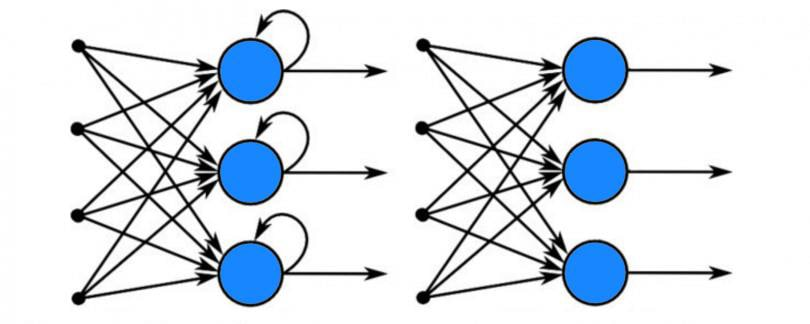
\includegraphics[width=0.75\columnwidth]{./img/recur.jpg}
\centering
\caption{Сравнение структуры рекуррентной нейронной сети (справа) и cети прямого распространения (слева). \cite{recur}}
\label{pic:recur}
\end{figure}

Нейроны сети производят вывод, а также копируют этот вывод и зацикливают его обратно на свой вход.
Так они получают информацию не только от предыдущего слоя, но и от самих себя предыдущего прохода. 
Это означает, что порядок, в котором подаются данные и обучается сеть, становится важным.

Большой проблемой при работе сетей RNN является проблема исчезающего градиента, которая заключается в быстрой потере информации с течением времени. 
Сети способны хранить только самую недавнюю информацию, что не всегда является достаточным для данной задачи. 
Допустим, мы хотим предсказать последнее слово в тексте “Я вырос в России… Мой родной язык русский”. 
Ближайший контекст предполагает, что последним словом будет называние языка, но, чтобы установить, 
какого именно языка, нам нужен контекст «России» из более отдаленного прошлого. Таким образом, 
разрыв между актуальной информацией и точкой ее применения может стать очень большим, что не всегда допустимо. 
В таких задачах необходимо уметь сохранять более глубокую память.

Сети с долгой краткосрочной памятью (Long Short Term Memory, LSTM) стараются решить вышеупомянутую проблему RNN потери информации. 
Для этого в сети используются фильтры и клетки памяти.

\begin{figure}[h]
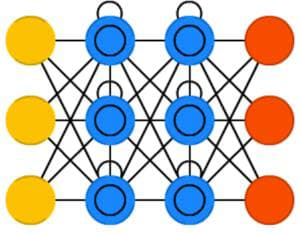
\includegraphics[width=0.75\columnwidth]{./img/recur_2.jpg}
\centering
\caption{Схема строения рекуррентной нейронной сети с долгой краткосрочной памятью}
\label{pic:recur_2}
\end{figure}

Память в LSTM называется ячейками (синие нейроны на рисунке  \ref{pic:recur_2} имеют в себе черный круг, 
символизирующий внутреннюю ячейку памяти). Помимо стандартной для 
рекуррентных нейронов передачи данных - принимают в качестве входных данных 
текущий входной параметр и предыдущее состояние - они имеют специальное внутреннее строение, 
что отличает их от обычной рекуррентной сети. 
Внутри у каждой клетки памяти есть три фильтра: входной, выходной и забывающий, которые решают, какую память сохранить и какую стереть.

\begin{figure}[h]
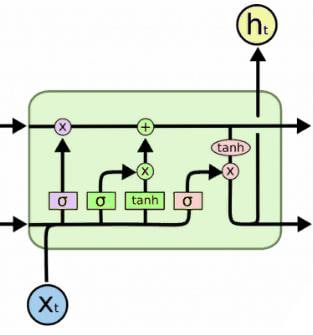
\includegraphics[width=0.75\columnwidth]{./img/recur_3.jpg}
\centering
\caption{Ячейка LSTM в развертке}
\label{pic:recur_3}
\end{figure}

На рисунке \ref{pic:recur_3} изображена ячейка LSTM в развертке. Обозначим 𝑥𝑡 - входное значение (голубой кружок), 
ℎ𝑡 – выходной вектор (желтый кружок). Ячейка состоит из нескольких компонентов, разделенных на три группы по цвету. 
Входной фильтр (компоненты зеленого цвета) определяет, сколько информации из предыдущего слоя будет храниться в клетке. 
Выходной фильтр (компоненты розового цвета) определяет, сколько информации получат следующие слои. 
Ну и забывающий фильтр (компоненты фиолетового цвета) – какую часть информации можно отсечь. 
Целью этих фильтров является защита информации внутри. 
Затем они объединяют предыдущее состояние, текущую память и входной параметр. 

Существуют различные модификации этой «классической» схемы ячейки. 
Сети LSTM способны научиться создавать более сложные структуры, чем классические рекуррентные сети. 
Решение задачи распознавания речи с использованием этой архитектуры было применено в исследовании \cite{2_recur}.

Двунаправленные RNN (Bidirectional Recurrent Neural Networks, BRNN) основаны на той идее, что выход в момент времени t может зависеть не только от предыдущих элементов
15 в последовательности, но и от будущих. Другими словами, сеть будет рассматривать данные как две последовательности – в прямом и в обратном направлении.
Двунаправленные рекуррентные нейронные сети (BRNN) соединяют два скрытых слоя, работающих в противоположных направлениях, 
с одним выходом, позволяя им получать информацию как из прошлых, так и из будущих состояний. 
BRNN разбивает нейроны классической рекуррентной сети на два направления, 
одно для прямых состояний (положительное направление времени), а другое для обратных состояний (отрицательное направление времени). 
Выходы из прямых состояний не связаны со входами обратных состояний, и наоборот. 
Это приводит к общей структуре, которую можно увидеть на рисунке ниже (сеть развернута на 4 временных шага).

Например, если нужно предсказать недостающее слово в середине последовательности (предложения), то нужно учитывать и левый, и правый контекст. 
Двунаправленная рекуррентная нейронная сеть представляет собой две рекуррентные сети, уложенные друг на друга. 
Без обратных состояний эта структура упрощается до обычной однонаправленной прямой RNN. 
Если прямые состояния исключены, получается классическая рекуррентная сеть с перевернутой временной осью.

\begin{figure}[h]
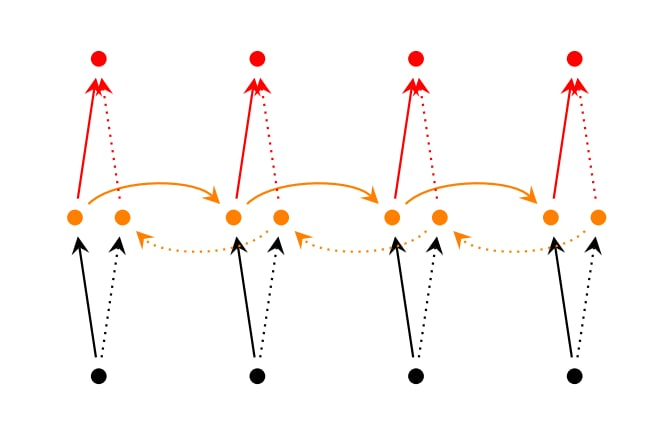
\includegraphics[width=0.75\columnwidth]{./img/recur_5.jpg}
\centering
\caption{Общая структура двунаправленной рекуррентной нейронной сети.}
\label{pic:recur_5}
\end{figure}


На рисунке \ref{pic:recur_5} изображена общая структура двунаправленной рекуррентной нейронной сети (BRNN). 
В процессе её обучения прямые и обратные состояния обрабатываются сначала в прямом проходе 
(на рисунке сплошной линией изображено положительное/прямое направление), выходные нейроны вычисляются последними 
(на рисунке пунктирной линией изображено отрицательное/обратное направление). 
При обратном проходе происходит обратное: сначала обрабатываются выходные нейроны, затем передаются состояния вперед и назад. 
Выход вычисляется на основе скрытого состояния обоих сетей RNN - веса обновляются только после завершения прямого и обратного проходов.

Двунаправленная рекуррентная нейронная сеть находит свое применение в задачи распознавания речи во многих успешных исследованиях \cite{3_recur}.

В последнее время для решения задачи распознавания речи обретает популярность \cite{4_recur}\cite{5_recur}\cite{6_recur} метод, 
использующий свёрточные нейронные сети. Архитектура сети изображена на рисунке \ref{pic:recur_6}.

\begin{figure}[h]
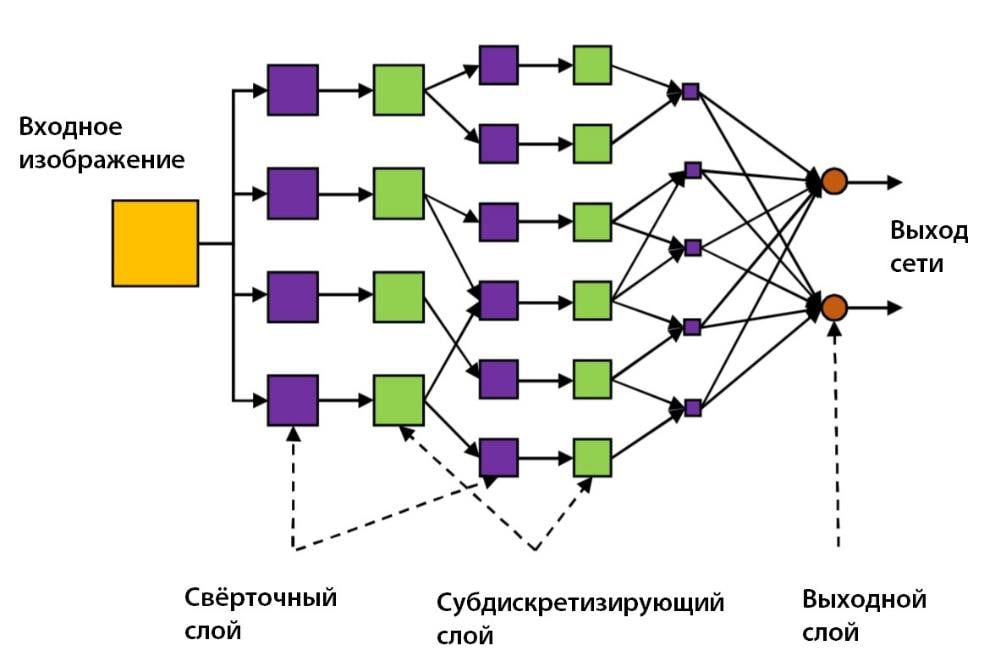
\includegraphics[width=0.75\columnwidth]{./img/recur_6.jpg}
\centering
\caption{Архитектура свёрточной нейронной сети}
\label{pic:recur_6}
\end{figure}

Для описания модели введем обозначения:
\begin{itemize}
  \item $l \in \left[1;L\right]$ - слой нейронной сети, где $L=2n+2$ – количество слоев в сети
  \item $a \in Z^{+}$ - количество скрытых слоёв в сети
  \item $N^l$ - количество карт признаков (фильтров) на слое $l$
  \item $y_n^l$ - $n$-ая карта признаков на слое $l$
\end{itemize}

Карта признаков является тензором и представляет собой выход после каждого слоя сети. 
К примеру, при применении N ядер (свёрток) к одному входному изображению получим N карт признаков. 
Обычно происходит чередование свёрточных и субдискретизирующих (пуллинга) слоёв. 
Тогда свёрточные слои стоят на нечётных позициях $l=1,3,…,2_n+1$, слои субдискретизации на четных позициях $l=2,4,…,2_n$.

Опишем устройство свёрточного слоя. Будем рассматривать слой $l$
, где $l$ принимается нечётный числом $l=1,3,…,2n+1$. Тогда для карты признаков $n$ введем следующие обозначения:

\begin{itemize}
  \item $w_{m,l}^l(i,j)$ – свёртка (ядро, фильтр), применяемая к карте признаков 𝑚 слоя $(l-1)$, на слое $l$ с картой признаков $n$;
  \item $b_n^l$ – пороговые значения, которые присоединяются к карте признаков $n$ на слое $l$;
  \item $V_n^l$ – список всех карт признаков слоя $(l-1)$, которые соединяются с картой признаков $n$ слоя $l$.
\end{itemize}

Таким образом, карта признаков $n$ свёрточного слоя $l$ будет вычисляться следующим образом:

\begin{equation}
  \begin{gathered}
    y_n^l = f_l (\sum_{m \in {V_n^l}} y_m^{l-1} \otimes W_{m,n}^l + b_n^l)
  \end{gathered}
  \label{eq:speach_formula_7}
\end{equation}

Где оператором $\otimes$ обозначена математическая операция двумерной свёртки. Пример вычисления изображен на \ref{pic:recur_7}.

\begin{figure}[h]
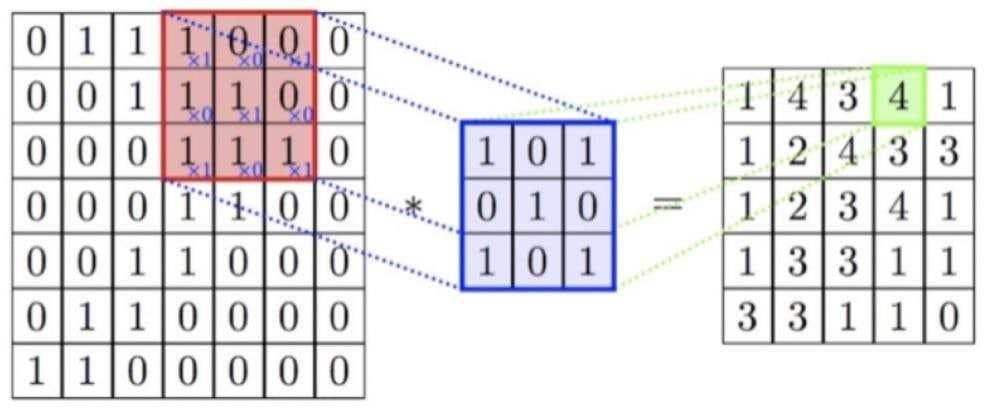
\includegraphics[width=0.75\columnwidth]{./img/recur_7.jpg}
\centering
\caption{Двумерная свёртка карты признаков (слева) и ядра (голубая матрица). \cite{7_recur}}
\label{pic:recur_7}
\end{figure}

Предположим, что размер входных карт признаков $y_m^{l-1}$ равен $H^{l-1} \times W^{l-1}$, 
а размер применяемой к ним свёртки $w_{m,n}^l$ равен $r^l \times c^l$. Тогда размер выходной карты признаков 𝓎𝑚𝑙 вычисляется как:

\begin{equation}
  \begin{gathered}
    (H^{l-1} - r^l + 1) \times (W^{l-1} - c^l + 1)
  \end{gathered}
  \label{eq:speach_formula_8}
\end{equation}

Подробная схема устройства слоя изображена на рисунке \ref{pic:recur_8}. 
Входная карта признаков представлена зеленым квадратом слева, свертка бежевым кругом, 
результат свертки – желтым квадратом. Затем, в случае многомерного фильтра 
(например, в случае работы с многоканальным изображением, когда каждый канал обрабатывается отдельно), 
результаты суммируются по формуле выше и применяется функция активации.
Иначе – желтый квадрат уже является ответом.

\begin{figure}[h]
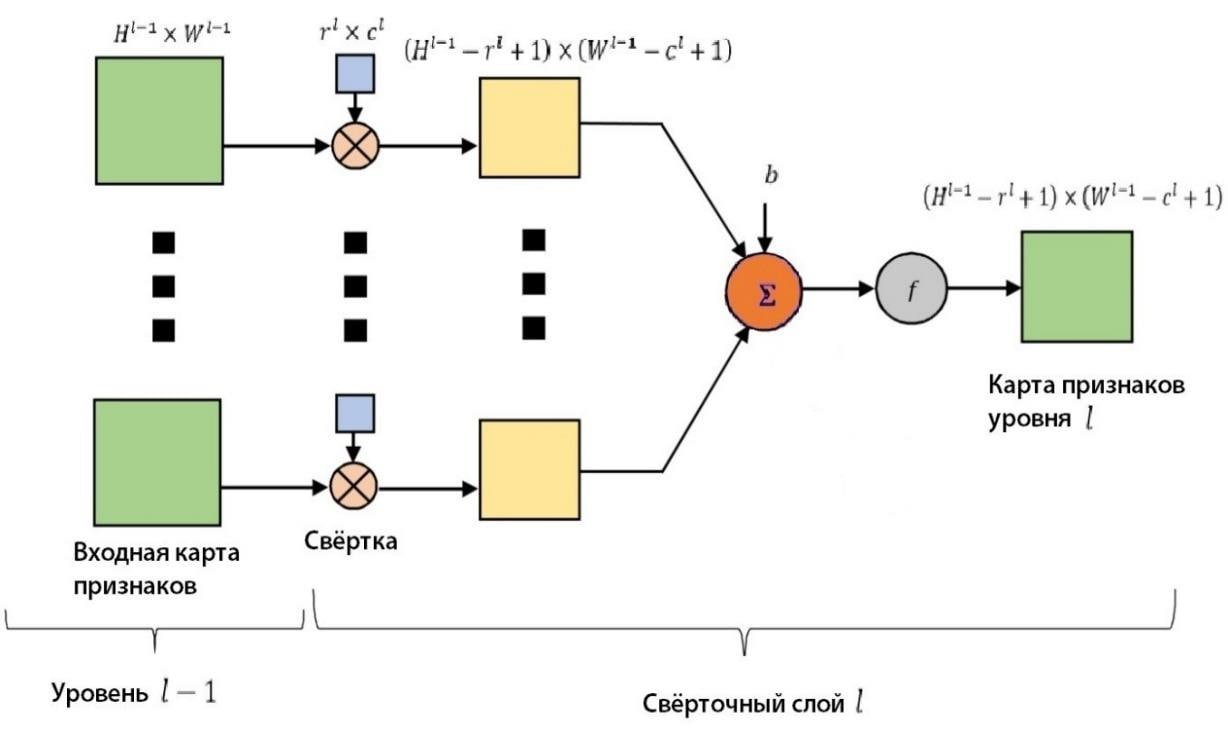
\includegraphics[width=0.75\columnwidth]{./img/recur_8.jpg}
\centering
\caption{Схема свёрточного слоя $l$}
\label{pic:recur_8}
\end{figure}

Введём в рассмотрение субдискретизирующий слой (пуллинговый). Его основная цель – уменьшение размерности входной карты признаков. 
В свёрточной нейронной сети номер $l$ субдискретизирующего слоя принято принимать чётный числом, то есть $l=2,4,…,2a$.

Разделим карту признаков $n (l-1)$ -ого слоя на непересекающиеся блоки размером 2x2 пикселя 
(Для простоты описания используется размер 2x2, однако на практике может использоваться и отличающийся размер). 
Затем просуммируем значения четырёх пикселей в каждом блоке и в результате получим матрицу $z_n^{l-1} = z_n^{l-1} = \left\{ z_n^{l-1}(i,j)\right\}$. 
Её элементами будут являться соответствующие значения сумм. 
Таким образом, формула для вычисления имеет следующий вид:

\begin{equation}
  \begin{gathered}
    z_n^{l-1} = y_n^{l-1}(2i - 1,2j - 1) + y_n^{l-1}(2i - 1,2j) + y_n^{l-1}(2i,2j - 1) + y_n^{l-1}(2i,2j)
  \end{gathered}
  \label{eq:speach_formula_9}
\end{equation}

Картой признаков $n$ субдискретизирующего слоя $l$ будет являться полученная матрица $z_n^{l-1}$. 
При этом вместо суммирования может использоваться любая другая функция (взятие максимума, взятие среднего, суммирование, разность и т.д.). 
Пример вычисления субдискретизирующего слоя с функцией взятия максимума и разбиением на блоки представлен на рисунке \ref{pic:recur_9}.

\begin{figure}[h]
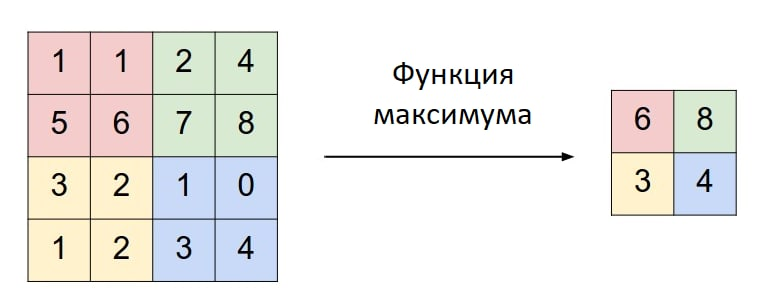
\includegraphics[width=0.75\columnwidth]{./img/recur_9.jpg}
\centering
\caption{Вычисление пуллингового слоя с функцией максимума и блоками 2x2. \cite{8_recur}}
\label{pic:recur_9}
\end{figure}

Таким образом, размер $H^l \times W^l$ карты признаков $y_n^l$ субдискретизирующего слоя $l$ при блоках 2x2 будет равен:

\begin{equation}
  \begin{gathered}
    H^l = \frac {H^{l-1}} {2} \\
    W^l = \frac {W^{l-1}} {2}
  \end{gathered}
  \label{eq:speach_formula_10}
\end{equation}

Существуют модификации слоя субдискретизации. Например, при разбиении карты признаков на блоки, последние могут перекрываться. 
Таким образом, можно задавать шаг смещения следующего блока относительно предыдущего. 
Другая модификация заключается в добавлении дополнительной «пустой рамки» к карте признаков. 
Так, при выполнении операции над блоком, оригинальные (не пустые) ячейки карты признаков могут вносить больший вклад в результат. 
Также, из-за добавления дополнительных ячеек выходная карта признаков будет иметь тот же размер, что и входная.

Выходной слой имеет номер $L=2a+2$, и состоит из $NL$ нейронов. 
Он представляет собой слой обычного многослойного персептрона. Формула для расчета значения выходного нейрона $n$:

\begin{equation}
  \begin{gathered}
    y_n^l = f_l (\sum_{m=1}^{N^{L-1}} y_m^{L-1} \otimes W_{m,n}^L + b_n^L)
  \end{gathered}
  \label{eq:speach_formula_11}
\end{equation}

Где:
\begin{itemize}
  \item $w_{m,n}^L$ – фильтр, применяемый к карте признаков 𝑚 последнего свёрточного слоя для получения перехода к нейрону $n$ выходного слоя (матрица весовых коэффициентов);
  \item $b_n^L$ – пороговое значение, добавляемое к нейрону $n$ (коэффициент сдвига).
\end{itemize}

Таким образом, выходом свёрточной нейронной сети является вектор следующего вида:

\begin{equation}
  \begin{gathered}
    y = \left[ y_1^L,y_1^L, ...,  y_{N^L}^L\right]
  \end{gathered}
  \label{eq:speach_formula_12}
\end{equation}

Для применения свёрточных сетей в задаче распознавания речи первоначально используется спектральное представление звукового потока.

\begin{figure}[h]
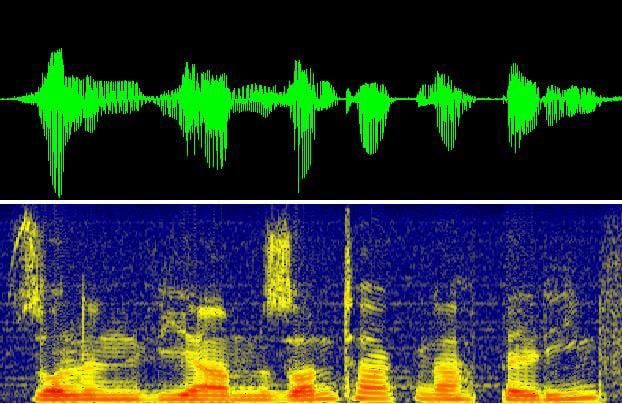
\includegraphics[width=0.75\columnwidth]{./img/recur_10.jpg}
\centering
\caption{ Изображение звуковой дорожки и соответствующего ей спектрального представления. Источник \cite{9_recur}}
\label{pic:recur_10}
\end{figure}

На основе полученного спектрального изображения (на рисунке \ref{pic:recur_10} изображена звуковая дорожка и соответствующее ей спектральное представление) 
стандартная свёрточная сеть для обработки спектрального представления сигнала выдает готовый распознанный результат.

\section{Семантический анализ текста и его виды}

Помимо анализа текста посредством опредения тональности текста, одним из типов анализа текста - является
семантический анализ текстов.

% тут надо нормально проставить cit
Семантический анализ текста – одна из основных проблем как 
теории создания систем искусственного интеллекта, относящаяся 
к обработке естественного языка (Natural Language Processing, NLP), так
и компьютерной лингвистики. В наш век компьютерных технологий
чрезвычайно важно получать информацию на естественном языке и
сделать так, чтобы эта информация могла перерабатываться с помощью
компьютера [4: 208]. 

На текущий момент выделяют следущие модели семантического анализа текста:
\begin{enumerate}
  \item Семантическая сеть
  \item Фреймовые модели
  \item Онтологическая модель
  \item Тезаурус 
\end{enumerate}

Семантическая сеть – модель предметной области, имеющая вид
ориентированного графа, вершины которого соответствуют объектам
предметной области, а дуги (ребра) задают отношения между ними.
Семантическая сеть появилась на основе математических формул. Семантическая сеть представляет собой схему, где есть концепты предметов, событий, состояний, с помощью линий показано отношение между
концептами.


Фреймовые модели – это структура, которая нужна для того, чтобы
описать понятия или ситуации, состоящая из характеристик этой ситуации и их значений. Фрейм можно считать элементом семантической
сети.

Онтологическая модель – это детальное описание какой-то предметной или проблемной области, которое можно использовать для
формулирования утверждений общего характера. Эта модель помогает
создавать понятия, которые впоследствии становятся пригодны для машинной обработки.

Тезаурус – лексический словарь, в котором показаны семантические отношения между лексическими единицами.
Благодаря этому словарю можно понять смысл, не только с помощью определения, но и соотнеся слова с другими понятиями и их группами, 
благодаря чему можно использовать искусственный интеллект для того, чтобы наполнить базы знаний. 
Обычно в тезаурусах используют такие семантические
отношения как, синонимы, антонимы, гипонимы, гиперонимы, меронимы, холонимы и паронимы. 
WordNet можно привести как пример тезауруса. 
Синсет (синонимический ряд) является основной словарной единицей WordNet, 
он объединяет слова с похожими значениями. Синсеты
это слова одной и той же части речи, что и слово, которое вы вводите. У
каждого такого слова есть своя дефиниция, которая объясняет значение
этого слова. Например, к слову ручка (pen) в таком словаре есть разные
значения: crayon, pencil, marker.

Из вышеперечисленного можно сделать вывод, что в век компьютеризации, 
вопрос о семантическом анализе текста становится все более
популярным. Из-за этого, область автоматической обработки текстов
сфокусировалась на прикладном аспекте. Семантический анализ представляет 
собой одну из сложных математических задач, несмотря на
востребованность практически во всех областях жизни современного
человека. Главной задачей является сделать так, чтобы компьютер смог
корректно трактовать образы, которые авторы текстов хотят передать
читателям или слушателям. 

%акустика
\section{Wav2vec}
Текущие современные модели распознавания речи требуют больших объемов расшифрованного звука.
Данные для достижения хороших результатов. В последнее время предобучение нейронных сетей
стал эффективным методом для условий, где размеченных данных недостаточно. Ключевая идея состоит в том, чтобы
изучить общие представления в установке, где имеется значительное количество размеченных или неразмеченных данных.
Доступны и использовать изученные представления для повышения производительности в последующей задаче.
для которых количество данных ограничено. Это особенно интересно для задач, где существенные
требуются усилия для получения помеченных данных, таких как распознавание речи.

В данный момент принято использовать предварительное обучение для для улучшения распознавания речи с учителем. Это
позволяет использовать немаркированные аудиоданные, которые гораздо проще собрать, чем помеченные данные.
Под предварительным обучением подразумевается факт обучения нейронной сети для задачи, в которой исользуется.
большой объем данных. 
Это широко применялось в "computer vision", обработке естественного языка и, в последнее время, для определенных речевых задач.

Предварительное обучение бывает: 

\begin{itemize}
  \item контролируемым образом
  \item в неконтролируемом режиме
\end{itemize}

Предварительное обучение похожа на трансферное обучение, когда вы предварительно обучаете модель, зная что есть $X$ и $y$.
Но для неконтролируемого предварительного обучения вы изучаете представление речи. 
wav2vec — это сверточная нейронная сеть (CNN), которая принимает необработанный звук 
в качестве входных данных и вычисляет общее представление, 
которое может быть введено в систему распознавания речи. 
Целью является контрастная потеря, которая требует отличить истинный будущий звуковой образец от негативов.

Учитывая контекст входного сигнала цель состоит в том, чтобы предсказать следующую обсервацию из этого образца речи.
Есть сопутствующая проблема, которая заключается в том, что следует иметь четкое представление как именно 
моделировать распределение $p(x)$ для речевых примеров. Решение это проблемы заключается в том что 
следует понизить размерность образцов речи при помощи "сети кодировщика", а уже затем использовать
контекстную сеть для прогнозирования следующих значений. 
wav2vec изучает представления аудиоданных, решая задачу прогнозирования контекста.

Конкретно $x_i \in X$
\begin{itemize}
 \item обучение первой сети кодировщика на основе CNN, которая мэпит X к Z
\end{itemize}

\begin{equation}
  \begin{gathered}
    f : X \rightarrow Z
  \end{gathered}
  \label{eq:speach_formula_12}
\end{equation}


\begin{itemize}
  \item обучение второй контекстной сети, также основанной на CNN, которая отображает Z к к одному контекстуальному тензору
\end{itemize}

\begin{equation}
  \begin{gathered}
    g : Z \rightarrow C
  \end{gathered}
  \label{eq:speach_formula_13}
\end{equation}

Представление этих двух сетей содержится на рисунке \ref{pic:wav}:

\begin{figure}[h]
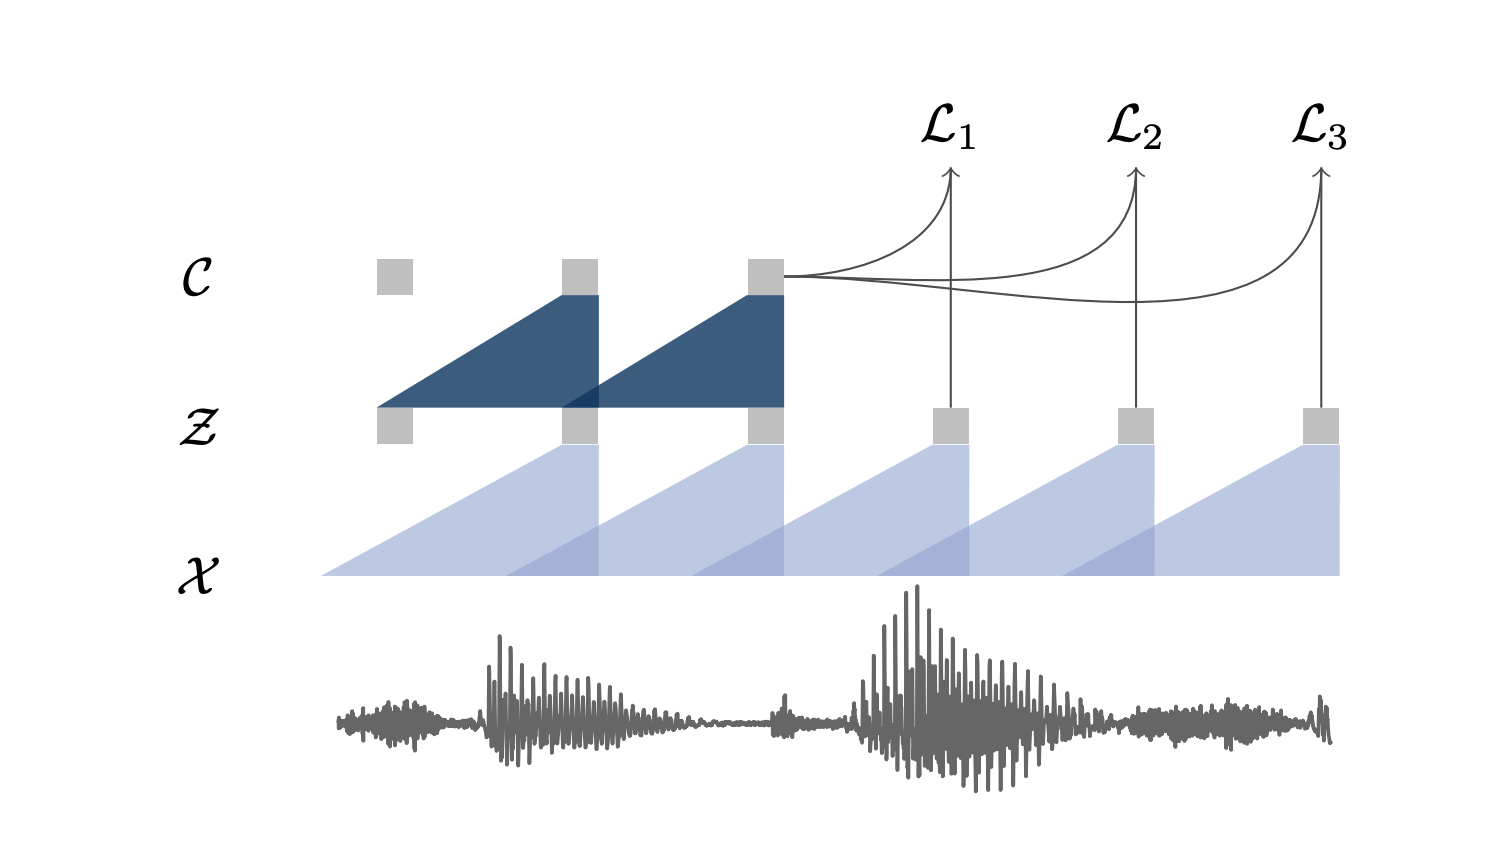
\includegraphics[width=0.75\columnwidth]{./img/wav_0.png}
\centering
\caption{Представление двух нейросетей}
\label{pic:wav}
\end{figure}
  
Вот подробности имплементации нейросетей: 
\begin{itemize}
  \item кодировщик представляет собой 5-слойную CNN с размерами ядра (10, 8, 4, 4, 4) и шагами (5, 4, 2, 2, 2) и охватывает 30 мс звука. Слои имеют 512 каналов, слой групповой нормализации и нелинейность ReLU.
  \item контекстная сеть имеет девять слоев с размером ядра три и шагом один, а общее рецептивное поле контекстной сети составляет около 210 мс. Слои имеют 512 каналов, слой групповой нормализации и нелинейный ReLU.
 \end{itemize}

Модель учат распознавать истинный образец $z_{i,k}, k$ шагов в будущем, от распределения предложения $p_n$, называемой констрастной потерей определяемой: 
\begin{equation}
  \begin{gathered}
    L_k = - \sum_{i = 1}^{T-k}(\log_\sigma(Z_{i+k}^t h_k (c_i)) + E_{z \sim p_n} \left[ \log_\sigma(- Z^{\sim T} h_k (c_i))\right])
  \end{gathered}
  \label{eq:speach_formula_14}
\end{equation}

Затем мы оптимизируются потери за несколько временных шагов:

\begin{equation}
  \begin{gathered}
    L_k = \sum_{k = 1}^{K} L_k
  \end{gathered}
  \label{eq:speach_formula_15}
\end{equation}

С целью получения ожидаемого распределения, отделяется условно десеть негативных 
примеров, выбирая одинаковые "триггер" факторы из этих негативных звуковых 
последовательностей. Другими словами, мы усредняется десять равномерно выбранных значений из разных аудиосэмплов.
$\lambda$ - количество негативных примеров.

Предсказывая следующие шаги, мы выполняется задача, называемая самостоятельным обучением речи.
Это также широко применяется в NLP и CV.

\section{k-nearest neighbors}

Метод $k$-ближайших соседей (англ. k-nearest neighbors algorithm, k-NN) — метрический 
алгоритм для автоматической классификации объектов или регрессии.
Это один из самых простых алгоритмов классификации.
Благодаря своей простоте, он является хорошим примером, 
с которого можно начать знакомство с областью Machine Learning. 
В данной статье рассмотрен пример написания кода такого 
классификатора на python, а также визуализация полученных результатов.

Для задач классификации метка класса присваивается на основе большинства голосов, 
т.е. используется метка, которая чаще всего представлена вокруг данной точки данных. 
Хотя технически это считается «многочисленным голосованием», термин «мажоритарное 
голосование» чаще используется в литературе. Различие между этими терминологиями 
заключается в том, что для «голосования большинством» технически требуется большинство, 
превышающее 50\%, что в первую очередь работает, когда есть только две категории. 
Когда у вас есть несколько классов, например. четыре категории, вам не обязательно нужно 50\%
голосов, чтобы сделать вывод о классе; вы можете присвоить метку класса при голосовании более 25\%.
Схема работы описана на рисунке \ref{pic:knn_diagramma}.

\begin{figure}[h]
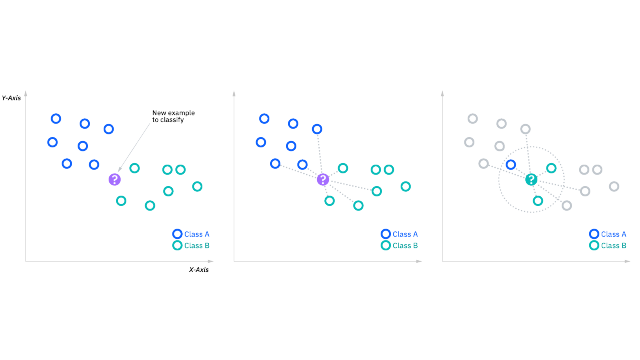
\includegraphics[width=0.75\columnwidth]{./img/knn_diagramma.png}
\centering
\caption{Диаграмма kNN}
\label{pic:knn_diagramma}
\end{figure}

В задачах регрессии используется та же концепция, что и в задачах классификации, 
но в этом случае для предсказания классификации берется среднее значение k ближайших соседей. 
Основное отличие здесь в том, что классификация используется для дискретных значений, 
а регрессия — для непрерывных. Однако, прежде чем можно будет провести классификацию, 
необходимо определить расстояние. Чаще всего используется евклидово расстояние, 
о котором мы поговорим ниже.

Напомним, что целью алгоритма k-ближайших соседей является определение ближайших соседей данной точки запроса, чтобы мы могли присвоить этой точке метку класса. Для этого у KNN есть несколько требований:

Определите свои показатели расстояния

Чтобы определить, какие точки данных находятся ближе всего к заданной точке запроса,
необходимо рассчитать расстояние между точкой запроса и другими точками данных. 
Эти метрики расстояния помогают формировать границы решений, которые разбивают точки
запроса на разные регионы. Обычно вы видите границы решений, визуализированные с помощью диаграмм Вороного.

Хотя есть несколько мер расстояния, которые вы можете выбрать, в этой статье будут рассмотрены только следующие:

Евклидово расстояние (p = 2): это наиболее часто используемая мера расстояния, 
и она ограничена векторами с действительными значениями. 
Используя приведенную ниже формулу, он измеряет прямую линию между точкой запроса и другой измеряемой точкой.

\begin{equation}
  \begin{gathered}
    d(x, y) = \sqrt{\sum_{i=1}^n(y_i-x_i)^2}
  \end{gathered}
  \label{eq:speach_formula_20}
\end{equation}

Манхэттенское расстояние (p = 1): это еще одна популярная метрика расстояния,
которая измеряет абсолютное значение между двумя точками. 
Его также называют расстоянием такси или расстоянием до городских кварталов, 
поскольку оно обычно визуализируется с помощью сетки, иллюстрирующей, 
как можно перемещаться от одного адреса к другому по улицам города.

\begin{equation}
  \begin{gathered}
    \text{M Distance} = d(x, y) = (\sum_{i=1}^m \left | x_i - y_i \right | )
  \end{gathered}
  \label{eq:speach_formula_21}
\end{equation}

Как и у любого алгоритма машинного обучения, у k-NN есть свои сильные и слабые стороны. 
В зависимости от проекта и приложения это может быть или не быть правильным выбором.

Плюсы данного подхода заключается в следующем: 
\begin{itemize}
  \item Простота реализации: учитывая простоту и точность алгоритма, это один из первых классификаторов, который выучит новый специалист по данным.
  \item Легко адаптируется: по мере добавления новых обучающих выборок алгоритм подстраивается под любые новые данные, поскольку все обучающие данные сохраняются в памяти.
  \item Несколько гиперпараметров: для KNN требуется только значение k и метрика расстояния, что является низким по сравнению с другими алгоритмами машинного обучения.
\end{itemize}

Минусы же выражены в следующем: 

\begin{itemize}
  \item Плохо масштабируется: поскольку KNN является ленивым алгоритмом, он занимает больше памяти и места для хранения данных по сравнению с другими классификаторами. Это может быть затратно как с точки зрения времени, так и денег. Больше памяти и хранилища повысит бизнес-расходы, а для обработки большего объема данных может потребоваться больше времени. Хотя для устранения неэффективности вычислений были созданы различные структуры данных, такие как Ball-Tree, в зависимости от бизнес-задачи может подойти другой классификатор.
  \item Алгоритм KNN имеет тенденцию становиться жертвой проблем размерности, что означает, что могут возникать проблемы с входными данными.
\end{itemize}

Однако минусы данного подхода могут быть нивелированы благодаря метода двойного расстояния, 
благодаря которому повышается точность распознавания. Тем самым kNN можно охарактеризовать как
хороший метрический алгоритм.

\section{Support Vector Machine}

В этой главе показана стратегия группировки звукоого знака с использованием новой методолгии
WOA-SVM и MapReduce. Система MapReduce выполняет анализ огромного объема информации 
(в данном случае аудиодокумента) с использованием преобразователя и редьюсера, 
где редуктор выполняет группировку с использованием ожидаемого классификатора WOA-SVM. 
Фундаментальные задачи по предложенному плану классификации аудио заключаются в следующем:

\begin{itemize}
  \item Улучшение модели извлечения бликов с восемью новыми бликами внесло свой вклад, как и области повторения, за исключением двух бликов пространства коэффициентов, которые созданы для эффективной классификации при анализе звука.
  \item Знакомство нового WOA-SVM с групповым звуковым флагом путем продвижения параметров SVM с помощью процедуры WOA.
  \item Исполнения рекомендуемого алгоритма классификации WOA-SVM на этапе MapReduce, поскольку аудиозаписи имеют гигантские размеры и лимит.
\end{itemize}

SVM \cite{svm} уникален для наиболее часто используемых классификаторов. Основная идея SVM состоит в том, 
чтобы изолировать различные классы, используя гиперплоскости. SVM достиг высоких показателей точности, 
когда информация прямо размечена. Как бы то ни было, представление SVM не может отделить непрямо 
реазмеченную информацию. Эту проблему можно решить, используя функции ядра, которые используются 
для изменения информации, одержимой другим многомерным пространством; отныне информация может быть выделена напрямую.
Выбор разумной функции ядра и изменение их ограничений — две основные трудности классификатора SVM. 
В этом сегменте будет представлено краткое описание идеи SVM в контексте группировки. 
Общая процедура работы алгоритма SVM пояснена на \ref{pic:svm_diagramma}.

\begin{figure}[h]
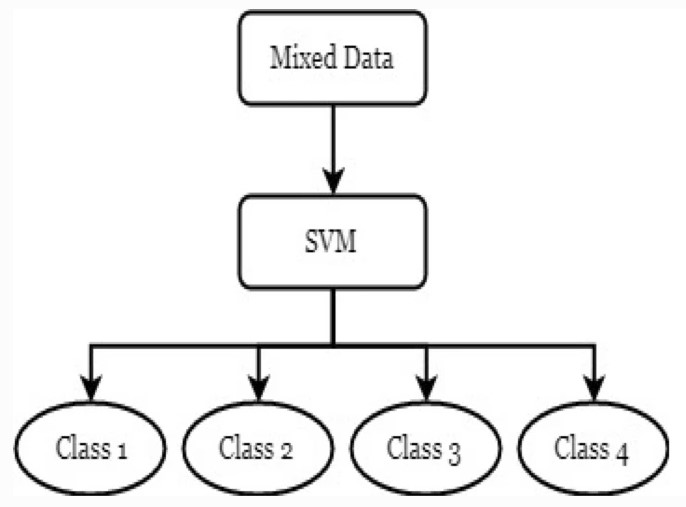
\includegraphics[width=0.75\columnwidth]{./img/svm_diagramma.jpg}
\centering
\caption{Базовые операции работы SVM}
\label{pic:svm_diagramma}
\end{figure}

Даны N линейно разделимых обучающих выборок, $X = \left \{ x_1, x_2, ..., x_N \right \}$ 
где $x_i$ это "итый" тренировочный сэмпл и каждая модель имеет $a$ харакетристик в 
бинаризированных классах $y \in \left \{ \pm 1 \right \}$. 

Линия $w^T x + b = 0$ обозначает границу произношения между двумя модулями, 
$w$ обозначает вектор весов, $b$ представляет собой смещение, 
а $b$ представляет собой предварительную модель.

Гиперплоскость делит Вселенную на два пространства. 
Цель состоит в том, чтобы найти оценку ω и b, 
чтобы расположить гиперплоскость так, чтобы она находилась 
за пределами того, что многие считают возможным из ближайших тестов, 
например опорных векторов (SV), и построить две плоскости, P1 и P2.

\section{Multi Layer Perceptron}
Многослойный персептрон (MLP) представляет собой полносвязный класс искусственных нейронных сетей с прямой связью (ANN). 
Термин MLP используется неоднозначно, иногда в широком смысле для обозначения любой ИНС с прямой связью, иногда 
строго для обозначения сетей, состоящих из нескольких уровней персептронов \cite{wiki_mlp}.

Обучение происходит в персептроне путем изменения веса соединения после обработки каждого фрагмента
данных в зависимости от количества ошибок в выходных данных по сравнению с ожидаемым результатом.

Мы можем представить степень ошибки в выходном узле $e_j(n) = d_j(n) - y_j(n)$, где $d$
целевое значение, а $y$ - значение, создаваемое персептроном.

\begin{equation}
  \begin{gathered}
    \varepsilon (n) = \frac{1}{2} \sum_j e_j^2
  \end{gathered}
  \label{eq:speach_formula_16}
\end{equation}

Используя градиентный спуск, изменение каждого веса равно:

\begin{equation}
  \begin{gathered}
    \Delta w_ji(n) = -\eta \frac{\partial \varepsilon_n}{\partial \upsilon_i (n)} y_i(n)
  \end{gathered}
  \label{eq:speach_formula_17}
\end{equation}

Где $y_i$ это это выход предыдущего нейрона, а $\eta$ – скорость обучения, 
которая выбирается таким образом, чтобы веса быстро сходились к ответу без колебаний.

Вычисляемая производная зависит от индуцированного локального поля $\upsilon_j$,
которое само изменяется. Легко доказать, что для выходного узла эту производную можно упростить до

\begin{equation}
  \begin{gathered}
    - \frac{\partial \varepsilon (n)}{\partial \upsilon_j (n)} = e_j(n) {\phi}'(\upsilon_j(n))
  \end{gathered}
  \label{eq:speach_formula_18}
\end{equation}

где ${\prime}'$ — производная описанной выше функции активации, которая сама по 
себе не меняется. Анализ более сложен для изменения весов в скрытом узле, 
но можно показать, что соответствующая производная равна

\begin{equation}
  \begin{gathered}
    - \frac{\partial \varepsilon (n)}{\partial \upsilon_j (n)} = {\phi}'(\upsilon_j(n)) \sum_k - \frac{\partial \varepsilon(n)}{\partial \upsilon_k(n)} \omega_kj(n)
  \end{gathered}
  \label{eq:speach_formula_19}
\end{equation}

Это зависит от изменения веса $k$-х узлов, которые представляют выходной слой. 
Таким образом, чтобы изменить веса скрытого слоя, веса выходного слоя изменяются 
в соответствии с производной функции активации, и поэтому этот алгоритм представляет собой обратное распространение функции активации.

\section{Выводы}


% В данном разделе была сформулирована постановка задачи, рассмотрены возможные ее решения с помощью архитектуры eBICA и подхода с использованием машинного обучения. 
% Выделен подход для распозвавания речи.

Было изучено описание работы модели виртуального актора. Изучены подходы и методы применительно к задаче распознавания речи.
Были рассмотрены ключевые подходы машинного обучения, которые будут использоваться в работе, а именно рекуррентные нейронные сети
